\documentclass[10pt, letterpaper]{article}

% Packages:
\usepackage[
    ignoreheadfoot, 
    top=2 cm, 
    bottom=2 cm, 
    left=2 cm, 
    right=2 cm, 
    footskip=1.0 cm, 
]{geometry} 
\usepackage{titlesec}
\usepackage{tabularx}
\usepackage{array}
\usepackage[dvipsnames]{xcolor}
\definecolor{primaryColor}{RGB}{0, 79, 144}
\usepackage{enumitem}
\usepackage{fontawesome5}
\usepackage{amsmath}
\usepackage[
    pdftitle={Mengfei Fan's CV},
    pdfauthor={Mengfei Fan},
    pdfcreator={LaTeX with RenderCV},
    colorlinks=true,
    urlcolor=primaryColor
]{hyperref}
\usepackage[pscoord]{eso-pic}
\usepackage{calc}
\usepackage{bookmark}
\usepackage{lastpage}
\usepackage{changepage}
\usepackage{paracol}
\usepackage{ifthen}
\usepackage{needspace}
\usepackage{iftex}
\usepackage{graphicx} % 用于插入照片

% Ensure that generated pdf is machine readable/ATS parsable:
\ifPDFTeX
    \input{glyphtounicode}
    \pdfgentounicode=1
    \usepackage[utf8]{inputenc}
    \usepackage{lmodern}
\fi

% Some settings:
\AtBeginEnvironment{adjustwidth}{\partopsep0pt}
\pagestyle{empty}
\setcounter{secnumdepth}{0}
\setlength{\parindent}{0pt}
\setlength{\topskip}{0pt}
\setlength{\columnsep}{0cm}
\makeatletter
\let\ps@customFooterStyle\ps@plain 
\patchcmd{\ps@customFooterStyle}{\thepage}{
    \color{gray}\textit{\small Mengfei Fan - Page \thepage{} of \pageref*{LastPage}}
}{}{}
\makeatother
\pagestyle{customFooterStyle}

\titleformat{\section}{\needspace{4\baselineskip}\bfseries\large}{}{0pt}{}[\vspace{1pt}\titlerule]

\titlespacing{\section}{
    -1pt
}{
    0.3 cm
}{
    0.2 cm
}

\renewcommand\labelitemi{$\circ$} 
\newenvironment{highlights}{
    \begin{itemize}[
        topsep=0.10 cm,
        parsep=0.10 cm,
        partopsep=0pt,
        itemsep=0pt,
        leftmargin=0.4 cm + 10pt
    ]
}{
    \end{itemize}
}

\newenvironment{highlightsforbulletentries}{
    \begin{itemize}[
        topsep=0.10 cm,
        parsep=0.10 cm,
        partopsep=0pt,
        itemsep=0pt,
        leftmargin=10pt
    ]
}{
    \end{itemize}
}

\newenvironment{onecolentry}{
    \begin{adjustwidth}{
        0.2 cm + 0.00001 cm
    }{
        0.2 cm + 0.00001 cm
    }
}{
    \end{adjustwidth}
}

\newenvironment{twocolentry}[2][]{
    \onecolentry
    \def\secondColumn{#2}
    \setcolumnwidth{\fill, 4.5 cm}
    \begin{paracol}{2}
}{
    \switchcolumn \raggedleft \secondColumn
    \end{paracol}
    \endonecolentry
}

\newenvironment{header}{
    \setlength{\topsep}{0pt}\par\kern\topsep\centering\linespread{1.5}
}{
    \par\kern\topsep
}

% Save the original href command in a new command:
\let\hrefWithoutArrow\href

% New command for external links:
\renewcommand{\href}[2]{\hrefWithoutArrow{#1}{\ifthenelse{\equal{#2}{}}{ }{#2 }\raisebox{.15ex}{\footnotesize \faExternalLink*}}}

\begin{document}
    \newcommand{\AND}{\unskip
        \cleaders\copy\ANDbox\hskip\wd\ANDbox
        \ignorespaces
    }
    \newsavebox\ANDbox
    \sbox\ANDbox{}

    \begin{header}
        \begin{tabular}{p{0.65\textwidth}p{0.35\textwidth}}
            \begin{flushleft}
                \textbf{\fontsize{28pt}{28pt}\selectfont Mengfei Fan}
                
                \vspace{0.5cm}
                
                \begin{tabular}{ll@{\hspace{1cm}}ll}
                    \faEnvelope[regular] & \hrefWithoutArrow{mailto:mengfeifan517@163.com}{mengfeifan517@163.com} & \faUniversity & Technical University of Munich \\
                    \faPhone* & \hrefWithoutArrow{tel:+49-162-8967744}{+49 1628967744} & \faGraduationCap & Master's in Mechatronics and Robotics \\
                    \faMapMarker* & Munich & \faLink & \hrefWithoutArrow{https://github.com/mengfei0517}{github.com/mengfei0517} \\
                    \faCalendar* & 1999-05 & \faSmileWink & Motion Control $|$ ML $|$ Robotics
                \end{tabular}
            \end{flushleft}
            & 
            \begin{flushright}
                \hspace{-15mm}
                \vspace{-15mm}
                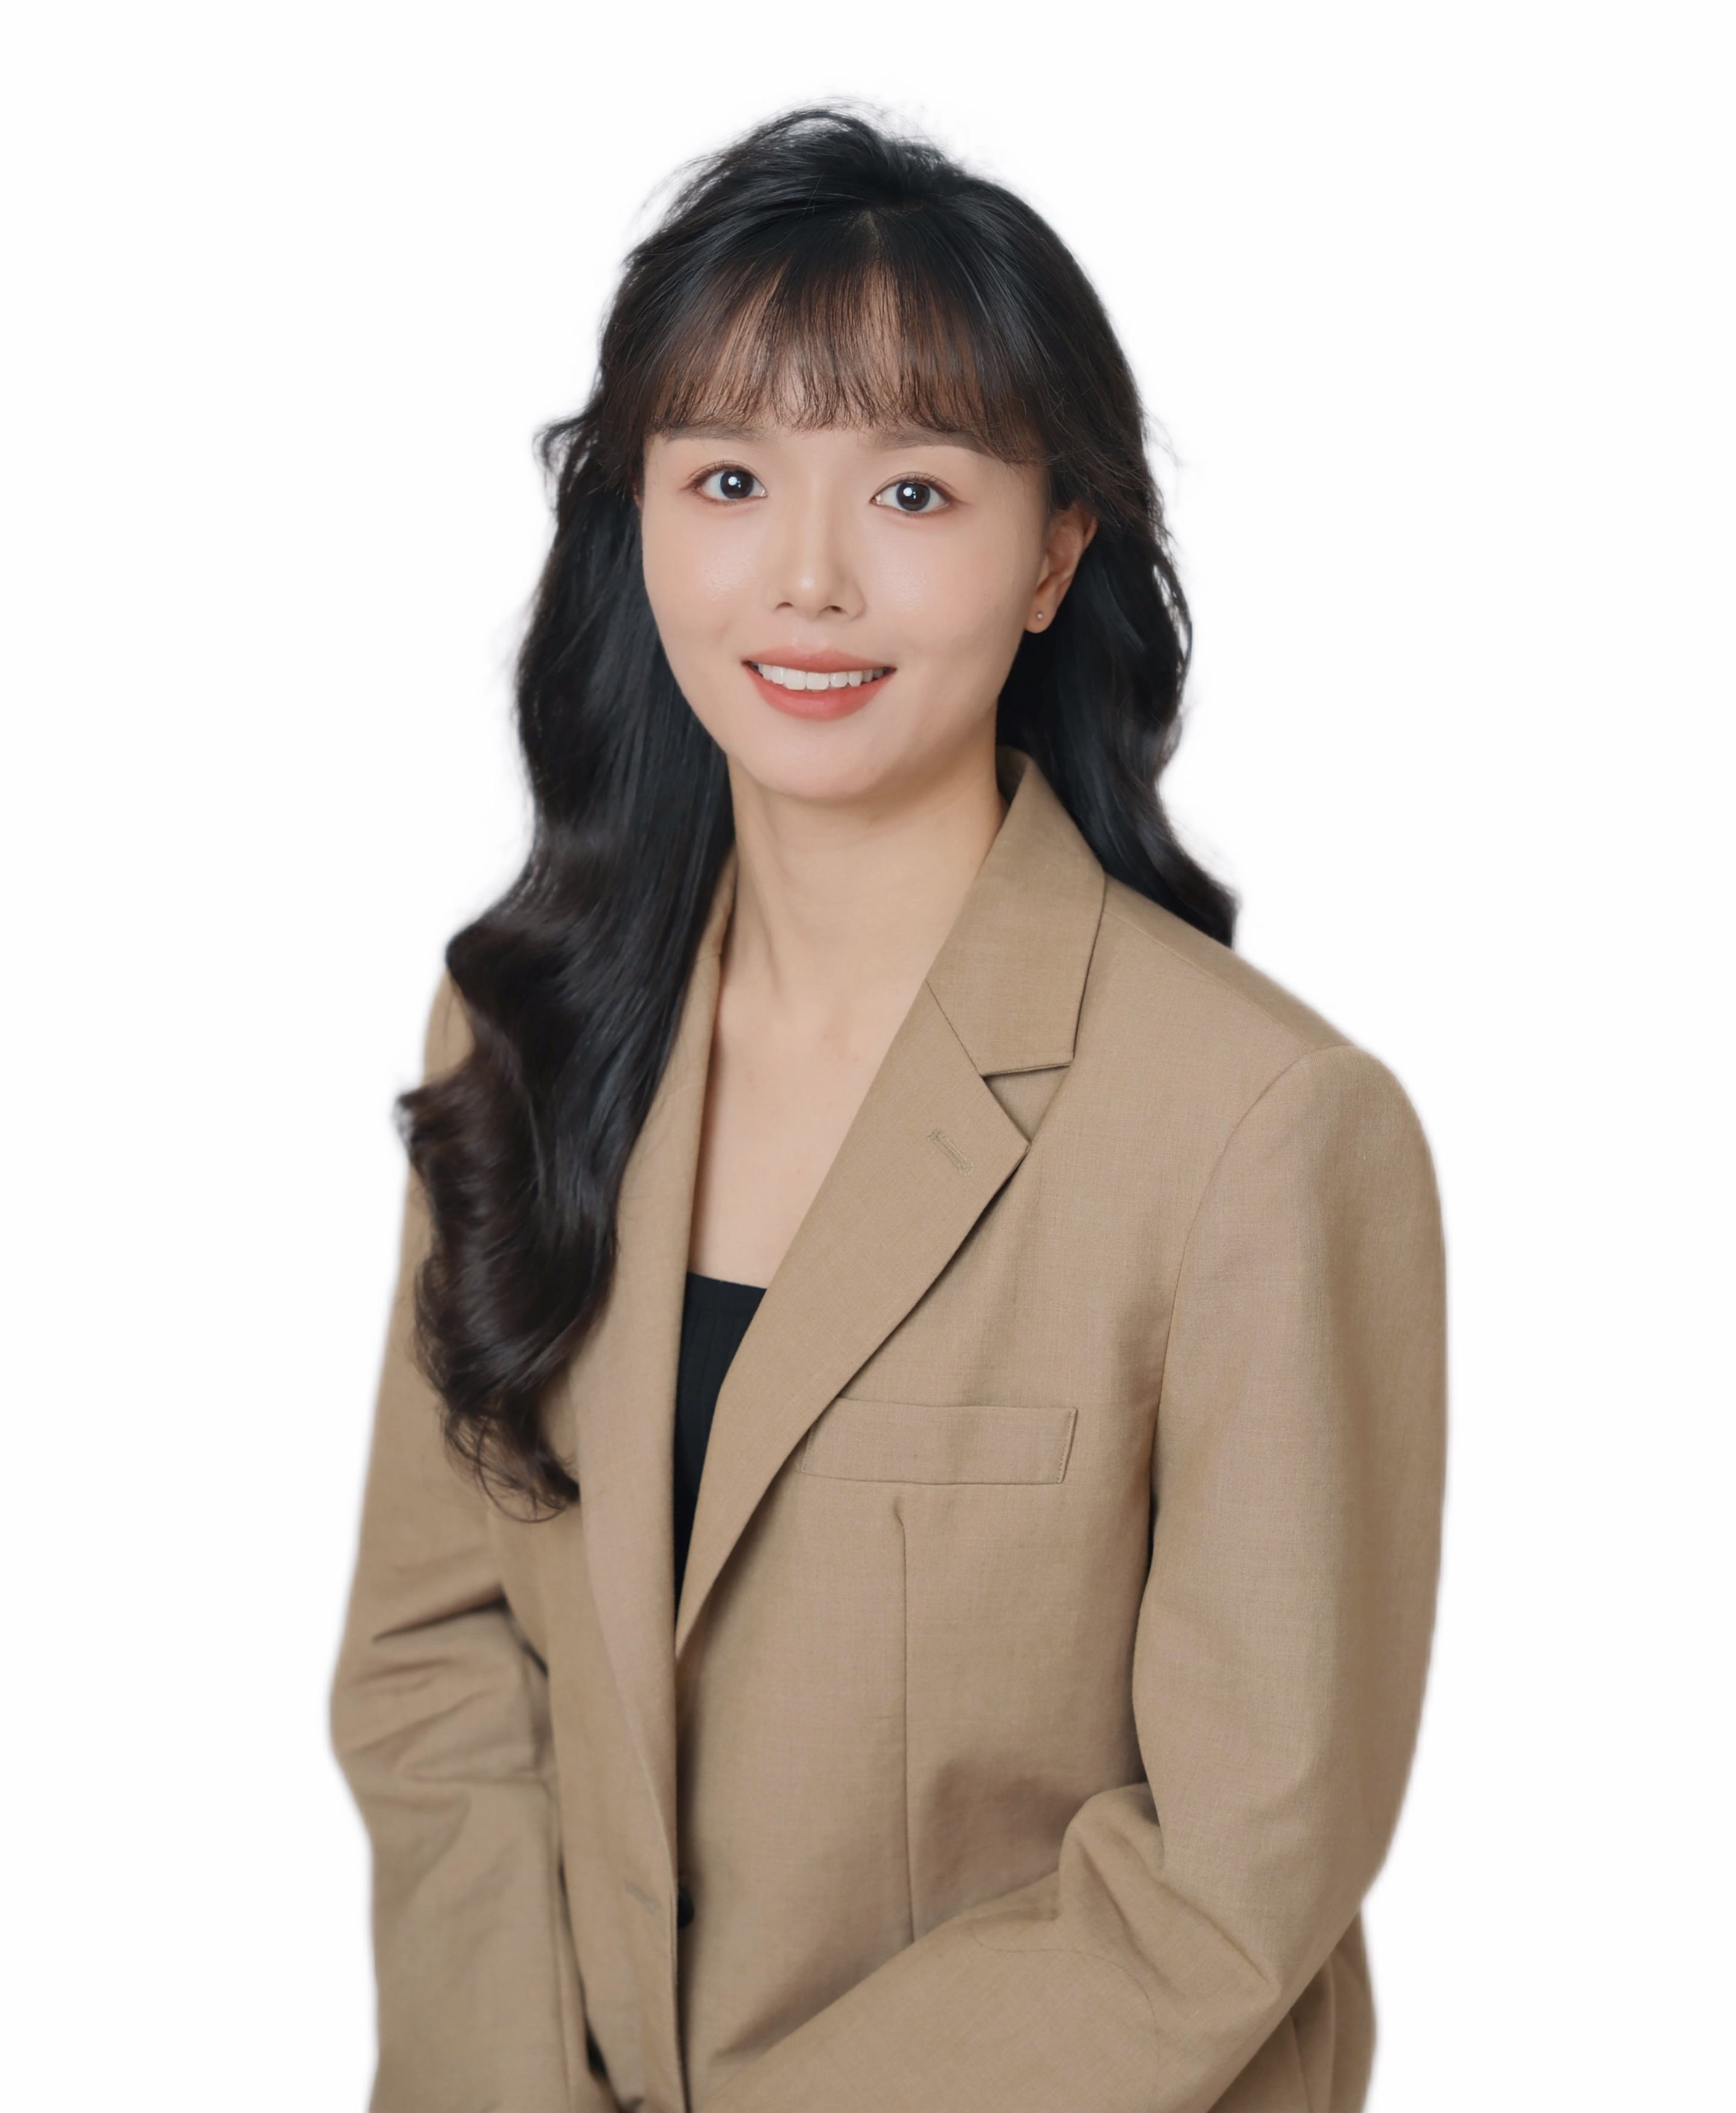
\includegraphics[width=3.5cm, height=4.2cm]{photo.jpg}
            \end{flushright}
        \end{tabular}
    \end{header}

    \vspace{0.3 cm}

    \section{Education}

    \begin{twocolentry}{\textit{Apr 2022 -- Jun 2025}}
        \textbf{Technical University of Munich (TUM)} \\
        \textit{Master's in Mechatronics and Robotics}
    \end{twocolentry}

    \vspace{0.10 cm}
    \begin{onecolentry}
        \begin{highlights}
            \item Representative Courses: Robot Dynamics, ROS/ROS2, Optimal Control, Machine Learning, Computational Intelligence
        \end{highlights}
    \end{onecolentry}

    \vspace{0.2 cm}

    \begin{twocolentry}{\textit{Sep 2017 -- Jun 2021}}
        \textbf{Sichuan University} \\
        \textit{Bachelor's in Mechanical Design, Manufacturing, and Automation}
    \end{twocolentry}

    \vspace{0.10 cm}
    \begin{onecolentry}
        \begin{highlights}
            \item National Scholarship, First Prize Scholarship
            \item Key Courses: Control Engineering, CNC Technology, Microcomputer Principles
        \end{highlights}
    \end{onecolentry}

    \vspace{0.3 cm}

    \section{Skills}

    \begin{onecolentry}
        \begin{highlights}
            \item \textbf{Programming:} C++17/20, Python, MATLAB
            \item \textbf{Robotics:} ROS1/2, MoveIt2, MuJoCo, Gazebo, Behaviour Trees, RL (PyTorch, SB3)
            \item \textbf{Control:} PID, MPC, LQR, IK, Trajectory Optimisation
            \item \textbf{Tools:} Linux, Git, VS Code, LaTeX
            \item \textbf{Languages:} Chinese (native), English (CET-6), German (C1)
        \end{highlights}
    \end{onecolentry}

    \vspace{0.3 cm}

    \section{Projects}

    \begin{twocolentry}{\textit{Apr 2024 -- Jun 2025}}
        \textbf{Long-Horizon Task Parsing \& Validation with LLMs and Behavior Trees} \\
        \textit{Python, LLMs, Behavior Trees, RoboCasa (MuJoCo), ROS2}
    \end{twocolentry}

    \vspace{0.10 cm}
    \begin{onecolentry}
        \begin{highlights}
            \item Built 3-layer LLM-based behavior tree task parser targeting robot actions, improving task success rate by ~15\% compared to baseline methods.
            \item Integrated predefined skill library with corresponding simulation platform for closed-loop execution in RoboCasa.
            \item Conducted systematic evaluation in high-fidelity kitchen simulation, achieving higher action executability and task success rates.
        \end{highlights}
    \end{onecolentry}

    \vspace{0.2 cm}

    \begin{twocolentry}{\textit{Jun 2024 -- Aug 2024}}
        \textbf{Autonomous Quadruped Robot Navigation} \\
        \textit{Linux, ROS, Unity, C++}
    \end{twocolentry}

    \vspace{0.10 cm}
    \begin{onecolentry}
        \begin{highlights}
            \item Integrated perception, path planning, trajectory planning, state machine, and control for quadruped robot obstacle avoidance navigation tasks.
            \item Implemented online and offline trajectory planning and coordinated motion planning with PID control integration.
            \item Optimized state machine and corresponding motion states to enable robust quadruped locomotion in challenging terrains.
        \end{highlights}
    \end{onecolentry}

    \vspace{0.2 cm}

    \begin{twocolentry}{\textit{July 2025}}
        \textbf{Multi-Object Pick-and-Place Task Execution Training} \\
        \textit{MuJoCo, Franka Panda, Linux, Python, Behavior Trees}
    \end{twocolentry}

    \vspace{0.10 cm}
    \begin{onecolentry}
        \begin{highlights}
            \item Implemented event-driven dense reward for Franka robot multi-object pick-and-place tasks and trained TQC agent in simulation.
            \item Wrapped RL sub-policies into BT action nodes, enabling robust sequencing across variable shelf heights.
            \item Implemented modular skill encapsulation (move, rotate, ee\_control) for clear task logic and debug-friendly execution.
        \end{highlights}
    \end{onecolentry}

    \vspace{0.2 cm}

    \begin{twocolentry}{\textit{Jan 2025 -- Mar 2025}}
        \textbf{Newton-Raphson Solver for Nonlinear Systems} \\
        \textit{Linux, C++}
    \end{twocolentry}

    \vspace{0.10 cm}
    \begin{onecolentry}
        \begin{highlights}
            \item Designed and implemented a high-performance Newton-Raphson solver in C++ to address nonlinear equations.
            \item Enhanced proficiency in object-oriented programming and numerical optimization techniques.
        \end{highlights}
    \end{onecolentry}

    \vspace{0.3 cm}

    \section{Experience}

    \begin{twocolentry}{\textit{Nov 2024 -- Apr 2025}}
        \textbf{Huawei 2012 Laboratories, Munich Research Center} \\
        \textit{Digital Engineer Working Student}
    \end{twocolentry}

    \vspace{0.10 cm}
    \begin{onecolentry}
        \begin{highlights}
            \item Automated cross-team workflows on DataLink platform; reduced hand-off time by 30\% and enhanced cross-department collaboration efficiency.
            \item Participated in robotics and intelligent automation digital transformation projects, responsible for logic orchestration, platform integration, and interface testing.
            \item Collaborated closely with Labs, HR, and Admin teams to optimize development processes and improve system maintainability and scalability.
        \end{highlights}
    \end{onecolentry}

    \vspace{0.2 cm}

    \begin{twocolentry}{\textit{\shortstack[l]{Nov 2022 -- Sep 2023\\Apr 2024 -- Sep 2024}}}
        \textbf{HiRain Technologies EU GmbH} \\
        \textit{Working Student, Munich}
    \end{twocolentry}

    \vspace{0.10 cm}
    \begin{onecolentry}
        \begin{highlights}
            \item Executed TSR perception tests; analysed model KPIs and drafted OEM reports.
            \item Analysed sensor data to evaluate perception model performance under diverse weather conditions.
            \item Provided project management support and prepared technical documentation for customer deliveries.
        \end{highlights}
    \end{onecolentry}

    \vspace{0.3cm}

    \begin{twocolentry}{\textit{Oct 2023 -- Mar 2024}}
        \textbf{HiRain Technologies Co., Ltd.} \\
        \textit{Intern, Beijing}
    \end{twocolentry}

    \vspace{0.10 cm}
    \begin{onecolentry}
        \begin{highlights}
            \item Developed EMB driver-intent recognition algorithm using MATLAB/Simulink; validated via MIL/SIL/VIL.
            \item Gained practical experience in embedded control systems and automotive functional safety workflows.
        \end{highlights}
    \end{onecolentry}

    \vspace{0.2 cm}

    \begin{twocolentry}{\textit{May 2021 -- Jul 2021}}
        \textbf{NIO Co., Ltd} \\
        \textit{Fellow Intern, Chengdu}
    \end{twocolentry}

    \vspace{0.10 cm}
    \begin{onecolentry}
        \begin{highlights}
            \item Developed a functional understanding of OEM-level autonomous driving features, including NIO Pilot and perception system architecture.
            \item Assisted the sales and R\&D interface team in aligning technical knowledge with customer requirements, contributing to customer satisfaction and product promotion.
            \item Participated in internal training and knowledge-sharing sessions, enhancing cross-department understanding of intelligent vehicle systems.
        \end{highlights}
    \end{onecolentry}

    \vspace{0.3 cm}

    \section{Additional Information}

    \begin{onecolentry}
        \begin{highlights}
            \item C1 German, Dual driver's licences (CN/DE)
            \item Certified top-rope climber
            \item China National Computer Level 2 (Microsoft Office)
            \item \href{https://www.linkedin.com/learning/certificates/9918408a208380a4de7ed2cb01fb073a890f95cd02fbb87258b295e1727d9a0a?trk=share_certificate}{Certificate of Completion: Career Essentials in Generative AI by Microsoft and LinkedIn}
            \item \textbf{Sports:} Fitness, Badminton, Skiing, Skateboarding, Running, Jazz Dance
            \item \textbf{Culinary:} Chinese \& Japanese Desserts, Bread Making, Innovative Cooking
        \end{highlights}
    \end{onecolentry}

\end{document}